

\let\textcircled=\pgftextcircled\chapter{Results and Evaluation}\label{chap:results}

\initial{T}his chapter will investigate the results generated from the modeling and reinforcement learning discussed in the previous chapters; it is structured to first present the outcomes of the training steps and hyperparameter tuning, followed by an in depth analysis of the training results and the agents learning process. Subsequent sections provide insights into the agents overall performance, including comparisons to human baselines, and a discussion of the practical deployment of a trained model. The chapter concludes with a critical evaluation of the project, discussing the extent to which the project aims were achieved and the potential for future work.


\section{Training Results}
% Training Results
% Present the learning curves for the agent, showing reward over time.
% Include a table or graph of the agent’s performance metrics at various checkpoints.
% Discuss any unexpected behaviours or anomalies observed during training.

The training scene used for the final training runs can be found in:
\newline
\texttt{Assets/Scenes/kiteboat\_training}. 
The final experimental setup was a combination of the best performing elements from the previous experiments.

This section presents the results of the hyperparameter tuning and the final training runs. It includes analyses of the learning curves, performance metrics, and unexpected behaviours observed during training.

\subsection{Hyperparameter Tuning}\label{sec:hyperparameter_tuning}

This subsection presents the findings from the grid search of hypereparameters, and the effect they had on the training runs. The goal was to identify the best combination of hyperparameters for this training application to then use for the final training runs. The dataset comprised 500 runs, each with a unique configuration file. The hyperparameters include \texttt{batch\_size}, \texttt{buffer\_size}, \texttt{learning\_rate}, \texttt{beta}, \texttt{epsilon}, \texttt{lambd}, \texttt{num\_epoch}, \texttt{hidden\_units}, \texttt{num\_layers}, \texttt{curiosity\_strength}, and \texttt{curiosity\_learning\_rate}. The performance was measured using the `Best Episode Length'- a metric that represents the duration for which the model successfully flew the kite while navigating towards the waypoint. 

A statistical summary was conducted to try and understand the most important tendencies of the data. The mean best episode length was found to be 5785 with a standard deviation of 7030, indicating a huge variability across different runs. A correlation matrix was computed to explore the linear relationship between the hyperparameters and the performance metric, the results of which can be seen in table$~$\ref{corr_matrix}. It was observed that \texttt{num\_epochs} had the strongest positive correlation (r=0.3007), suggesting a tendency for longer episodes with more epochs. On the other hand \texttt{batch\_size} and \texttt{epsilon} showed a negative correlation (r=-0.3007 and r=-0.3007 respectively) to the episode length.

\begin{table}[!htb]
    \centering
    \begin{tabular}{c|c}
        \textbf{Hyperparameter} & \textbf{Correlation} \\
        \hline

        \texttt{num\_epoch} & 0.3007 \\
        \texttt{buffer\_size} & 0.2640 \\
        \texttt{num\_layers} & 0.1246 \\
        \texttt{Av Loss} & 0.0973 \\
        \texttt{lambd} & 0.0964 \\
        \texttt{beta} & 0.0424 \\
        \texttt{curiosity\_strength} & -0.0074 \\
        \texttt{hidden\_units} & -0.0185 \\
        \texttt{curiosity\_learning\_rate} & -0.1168 \\
        \texttt{learning\_rate} & -0.1168 \\
        \texttt{epsilon} & -0.1258 \\
        \texttt{batch\_size} & -0.2275 \\
        \bottomrule
    \end{tabular}
    \caption{Correlation matrix of hyperparameters}\label{corr_matrix}
\end{table}

% A visualization of the relationships and distributions within the data was created and can be seen in figure$~$\ref{vis_matrix}. Scatter plot matrices were generated using \texttt{Seaborn} and \texttt{Matplotlib} libraries in Python to display the best pairwise relationships between the most correlated hyperparameters and the best episode length. Also included in figure$~$\ref{vis_matrix} are bar plots, which represent the feature importance derived from a Random Forest Model$~$\cite{randomforrestM}. 

A Random Forrest Regressor$~$\cite{randomforrestM} was utilised to estimate the importance of each hyperparameter in predicting the best episode length. The model was trained on a subset of the data and validated using a test set, resulting in a Mean Squared Error (MSE) of 53 million. This very large value indicates significant variability and suggests the model's performance is highly sensitive to changing hyperparameters. Figure$~$\ref{feature_importance} shows the feature importance bar plot, which emphasises the significance of \texttt{num\_epochs} and \texttt{buffer\_size} in the model's success. The \texttt{analysis.py} script, that performs the above calculations can be found in section$~$\ref{sec:analysis} of the appendices.

% \begin{figure}[!htb]
%     \centering
%     \resizebox{\textwidth}{!}{%
%     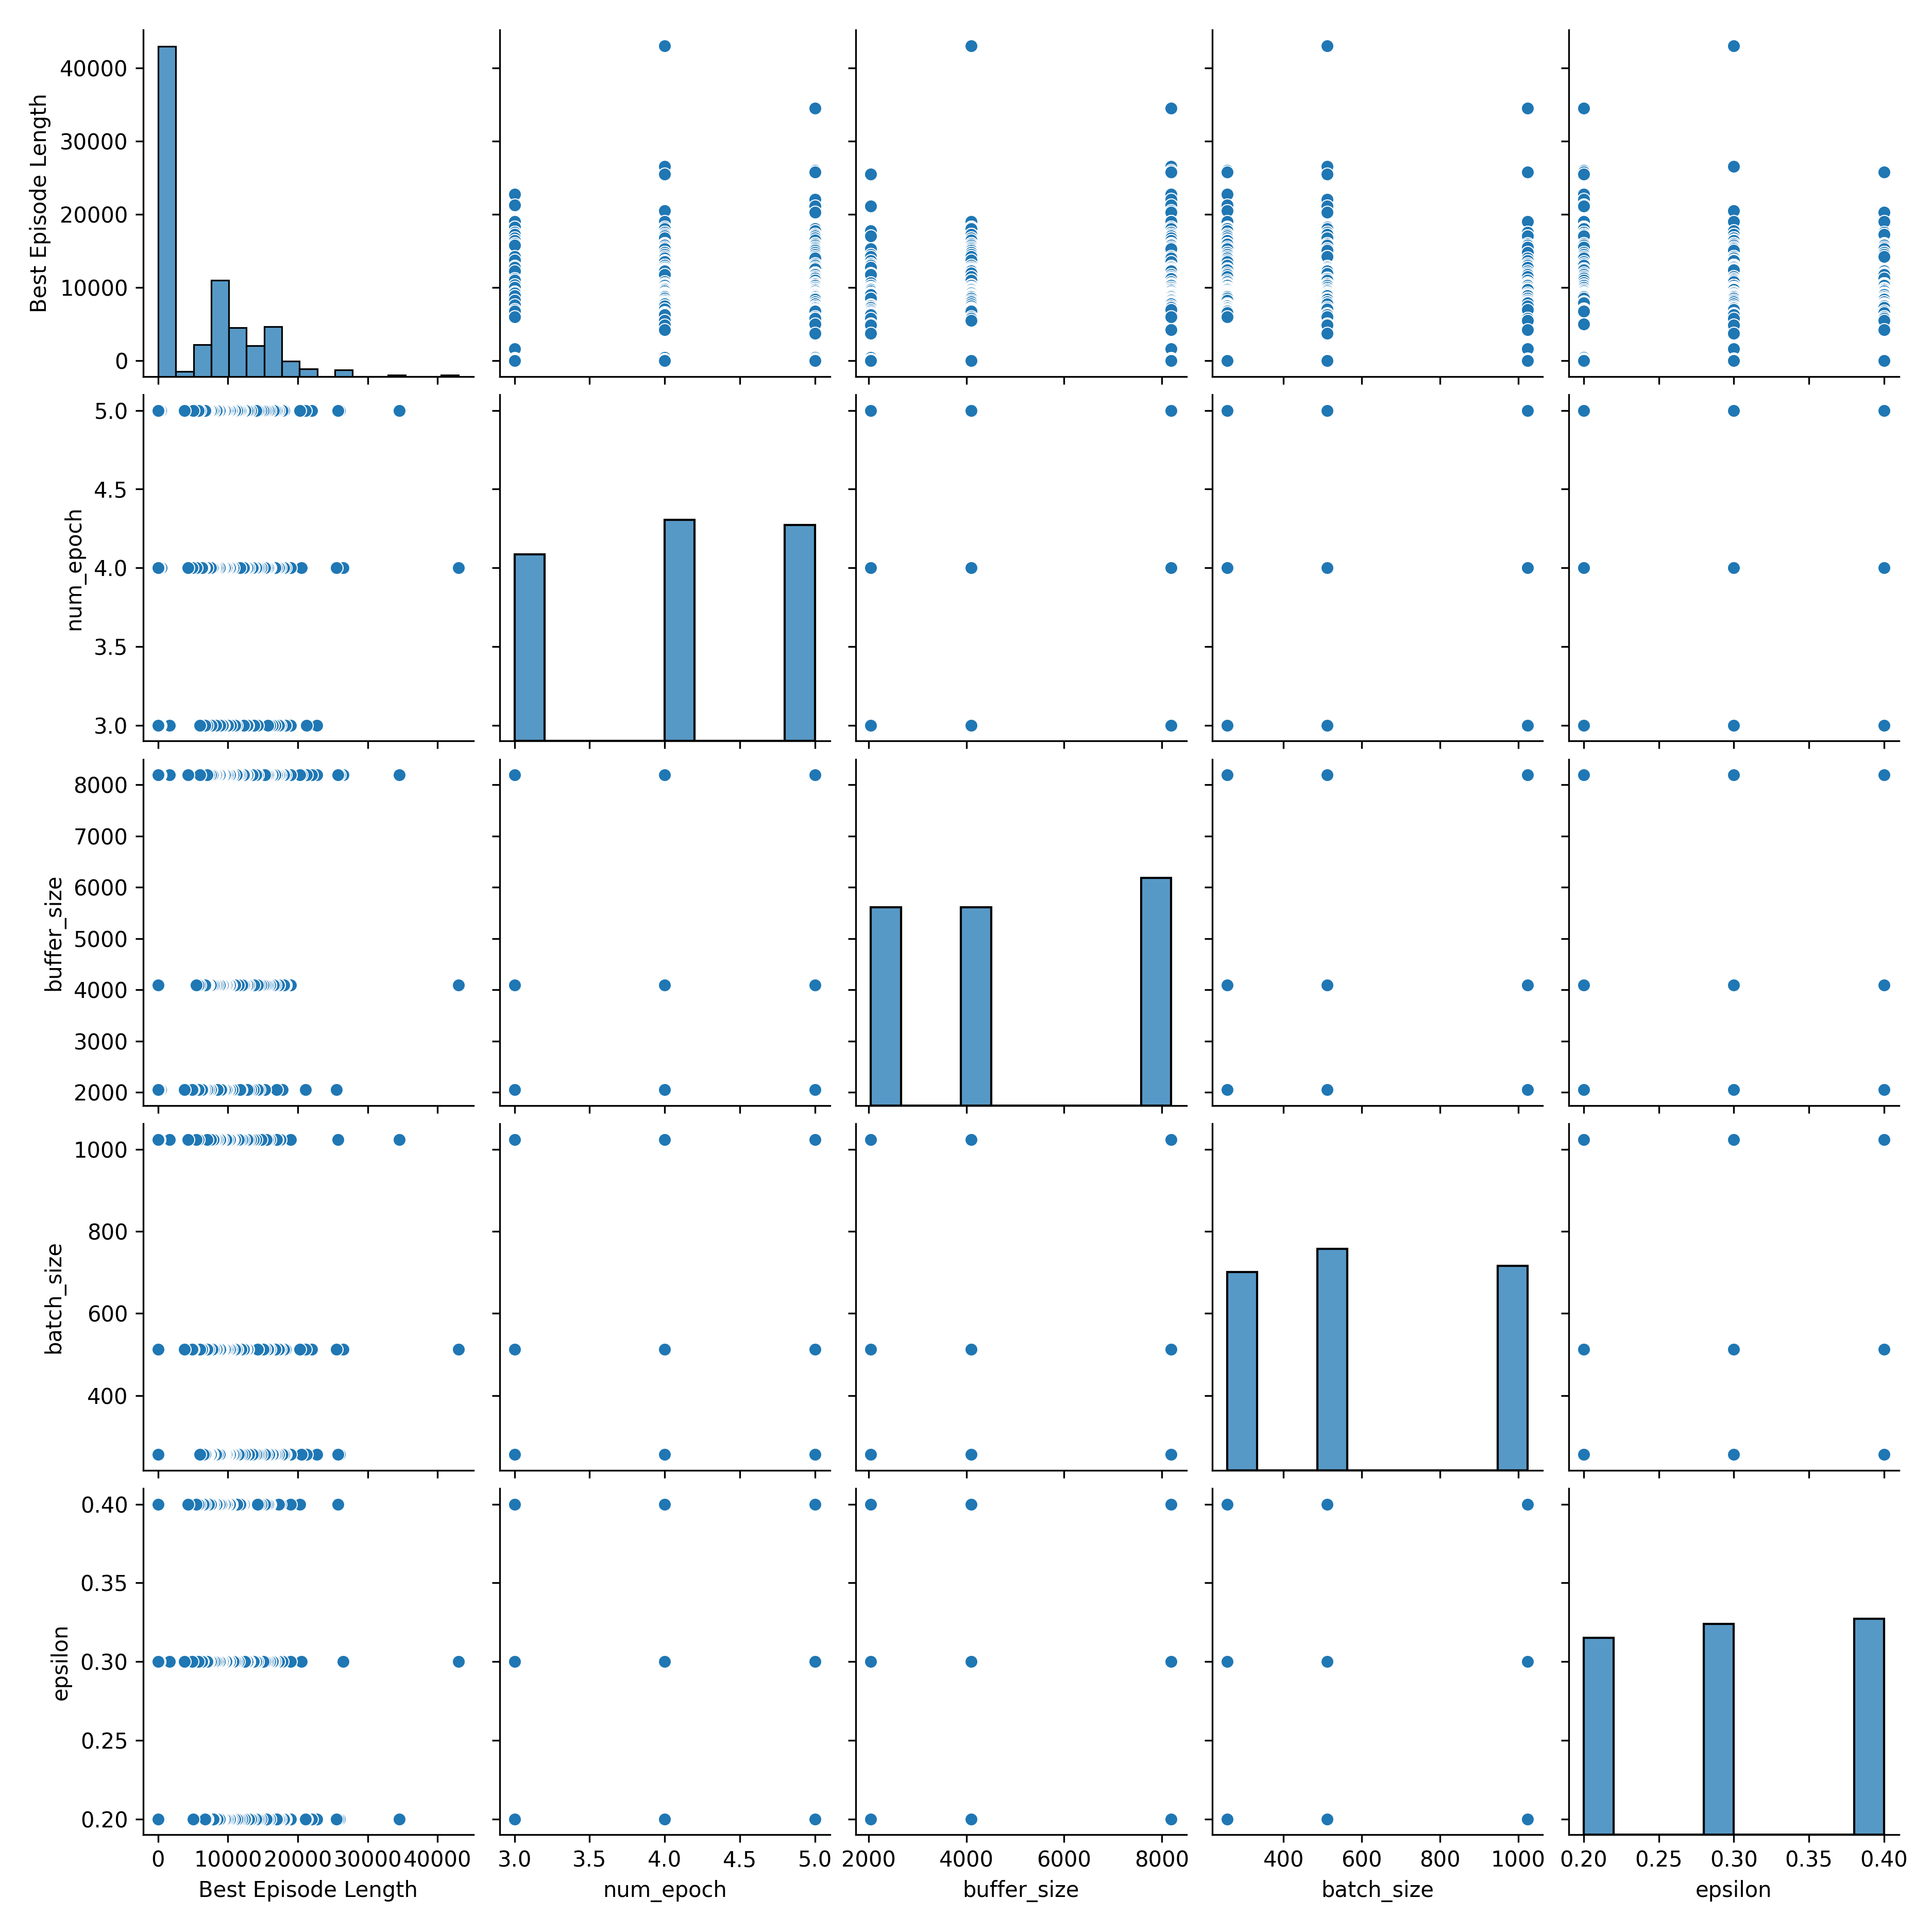
\includegraphics[]{Images/scatter_plot_matrix.png}
%     }
%     \caption{Visualization matrix of hyperparameters}\label{vis_matrix}
% \end{figure}

\begin{figure}[!htb]
    \centering
    \resizebox{\textwidth}{!}{%
    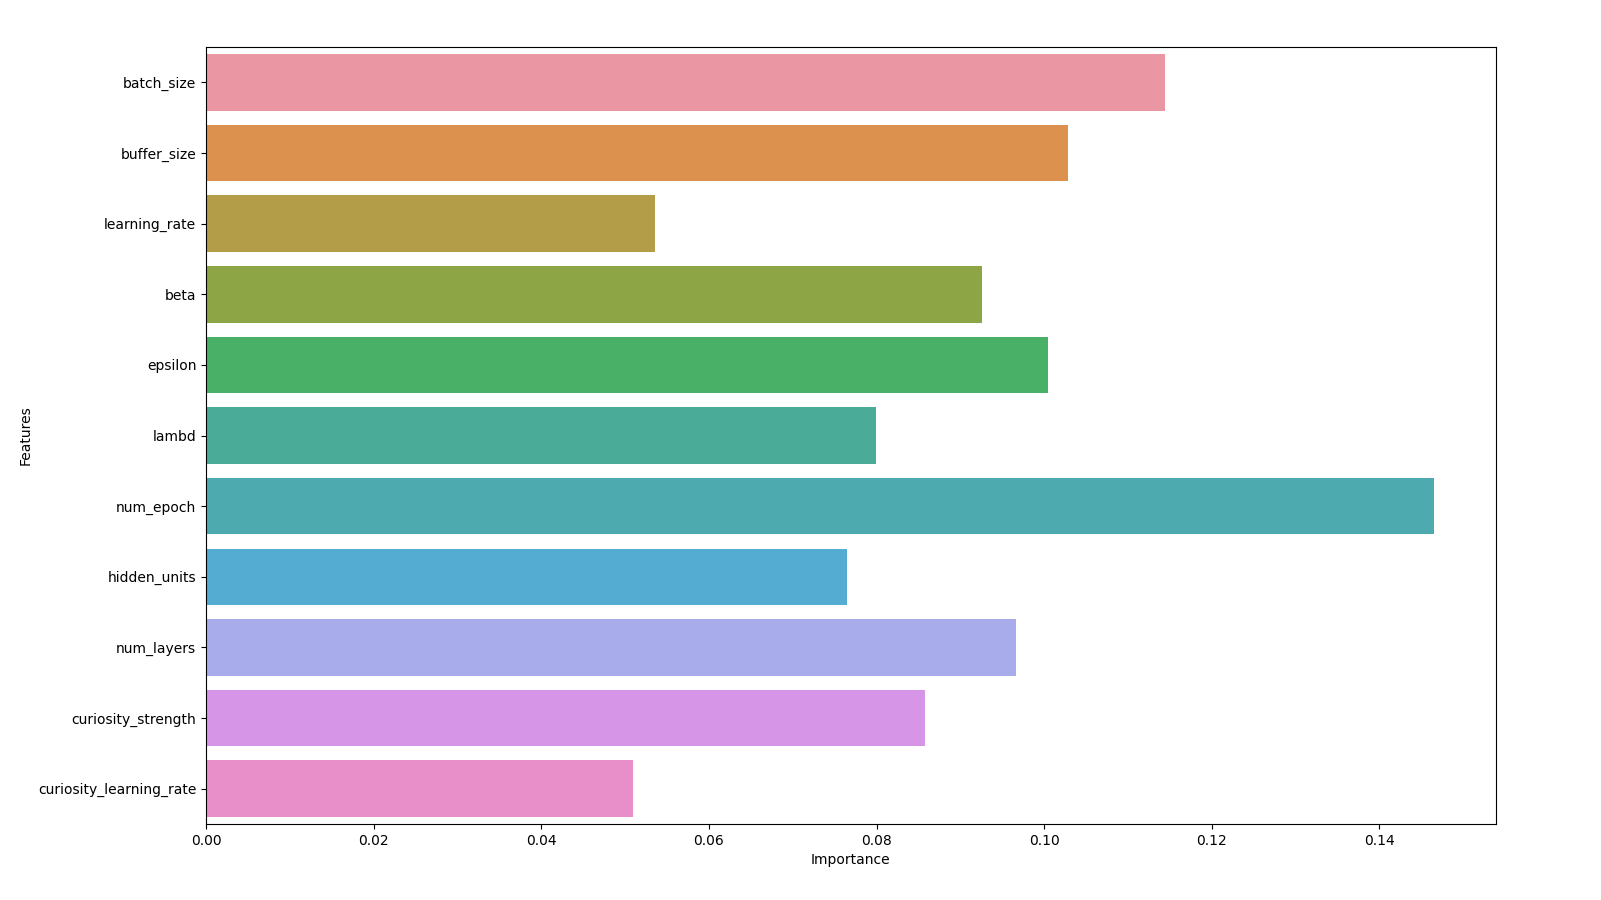
\includegraphics[]{Images/feature_importance.png}
    }
    \caption{Feature importance of hyperparameters}\label{feature_importance}
\end{figure}

% After training was complete, the results were extracted and a linear regression model was created to illuminate which of the changing hyperparameter values had the greatest impact on the performance metric, in this case episode length, for this a python script was used REF APENDIX. The results of the linear regression model can be seen in Figure~\ref{regression}. The coefficients derived from the regression, depicted in the bar chart, offer a visual representation of the impact each hyperparameter had on the performance metric. Notably, the \texttt{learning\_rate}, \texttt{beta}, and \texttt{curiosity\_learning\_rate} had the greatest impact on the performance metric. This suggests that a smaller learning rate reduces the strength of the updates to the policy, and thus the agent learns slower, but more reliably for a complex task. Increasing the value of the \texttt{beta} hyperparameter, which is the strength of the entropy regularization term, also had a positive impact on the performance metric. This suggests that the agent was able to learn more effectively when the policy was encouraged to explore more.

In hindsight, incorporating a dynamic learning rate that varies throughout the training phase would have been beneficial i.e scheduling it to change over the course of the training run. This approach would involve initiating the training with a relatively high learning rate, thereby facilitating rapid learning in the initial stages. As the training progressed, gradually reducing the learning rate would allow the agent to fine tune its policy without unlearning previously learned behaviours, which is a common problem with RL agents. Moreover, employing an non-linear learning rate schedule could have provided a more controlled reduction in pace, enhancing the stability in the latter stages of the training. 


% \begin{figure}
%     \centering
%     \resizebox{\textwidth}{!}{%
%     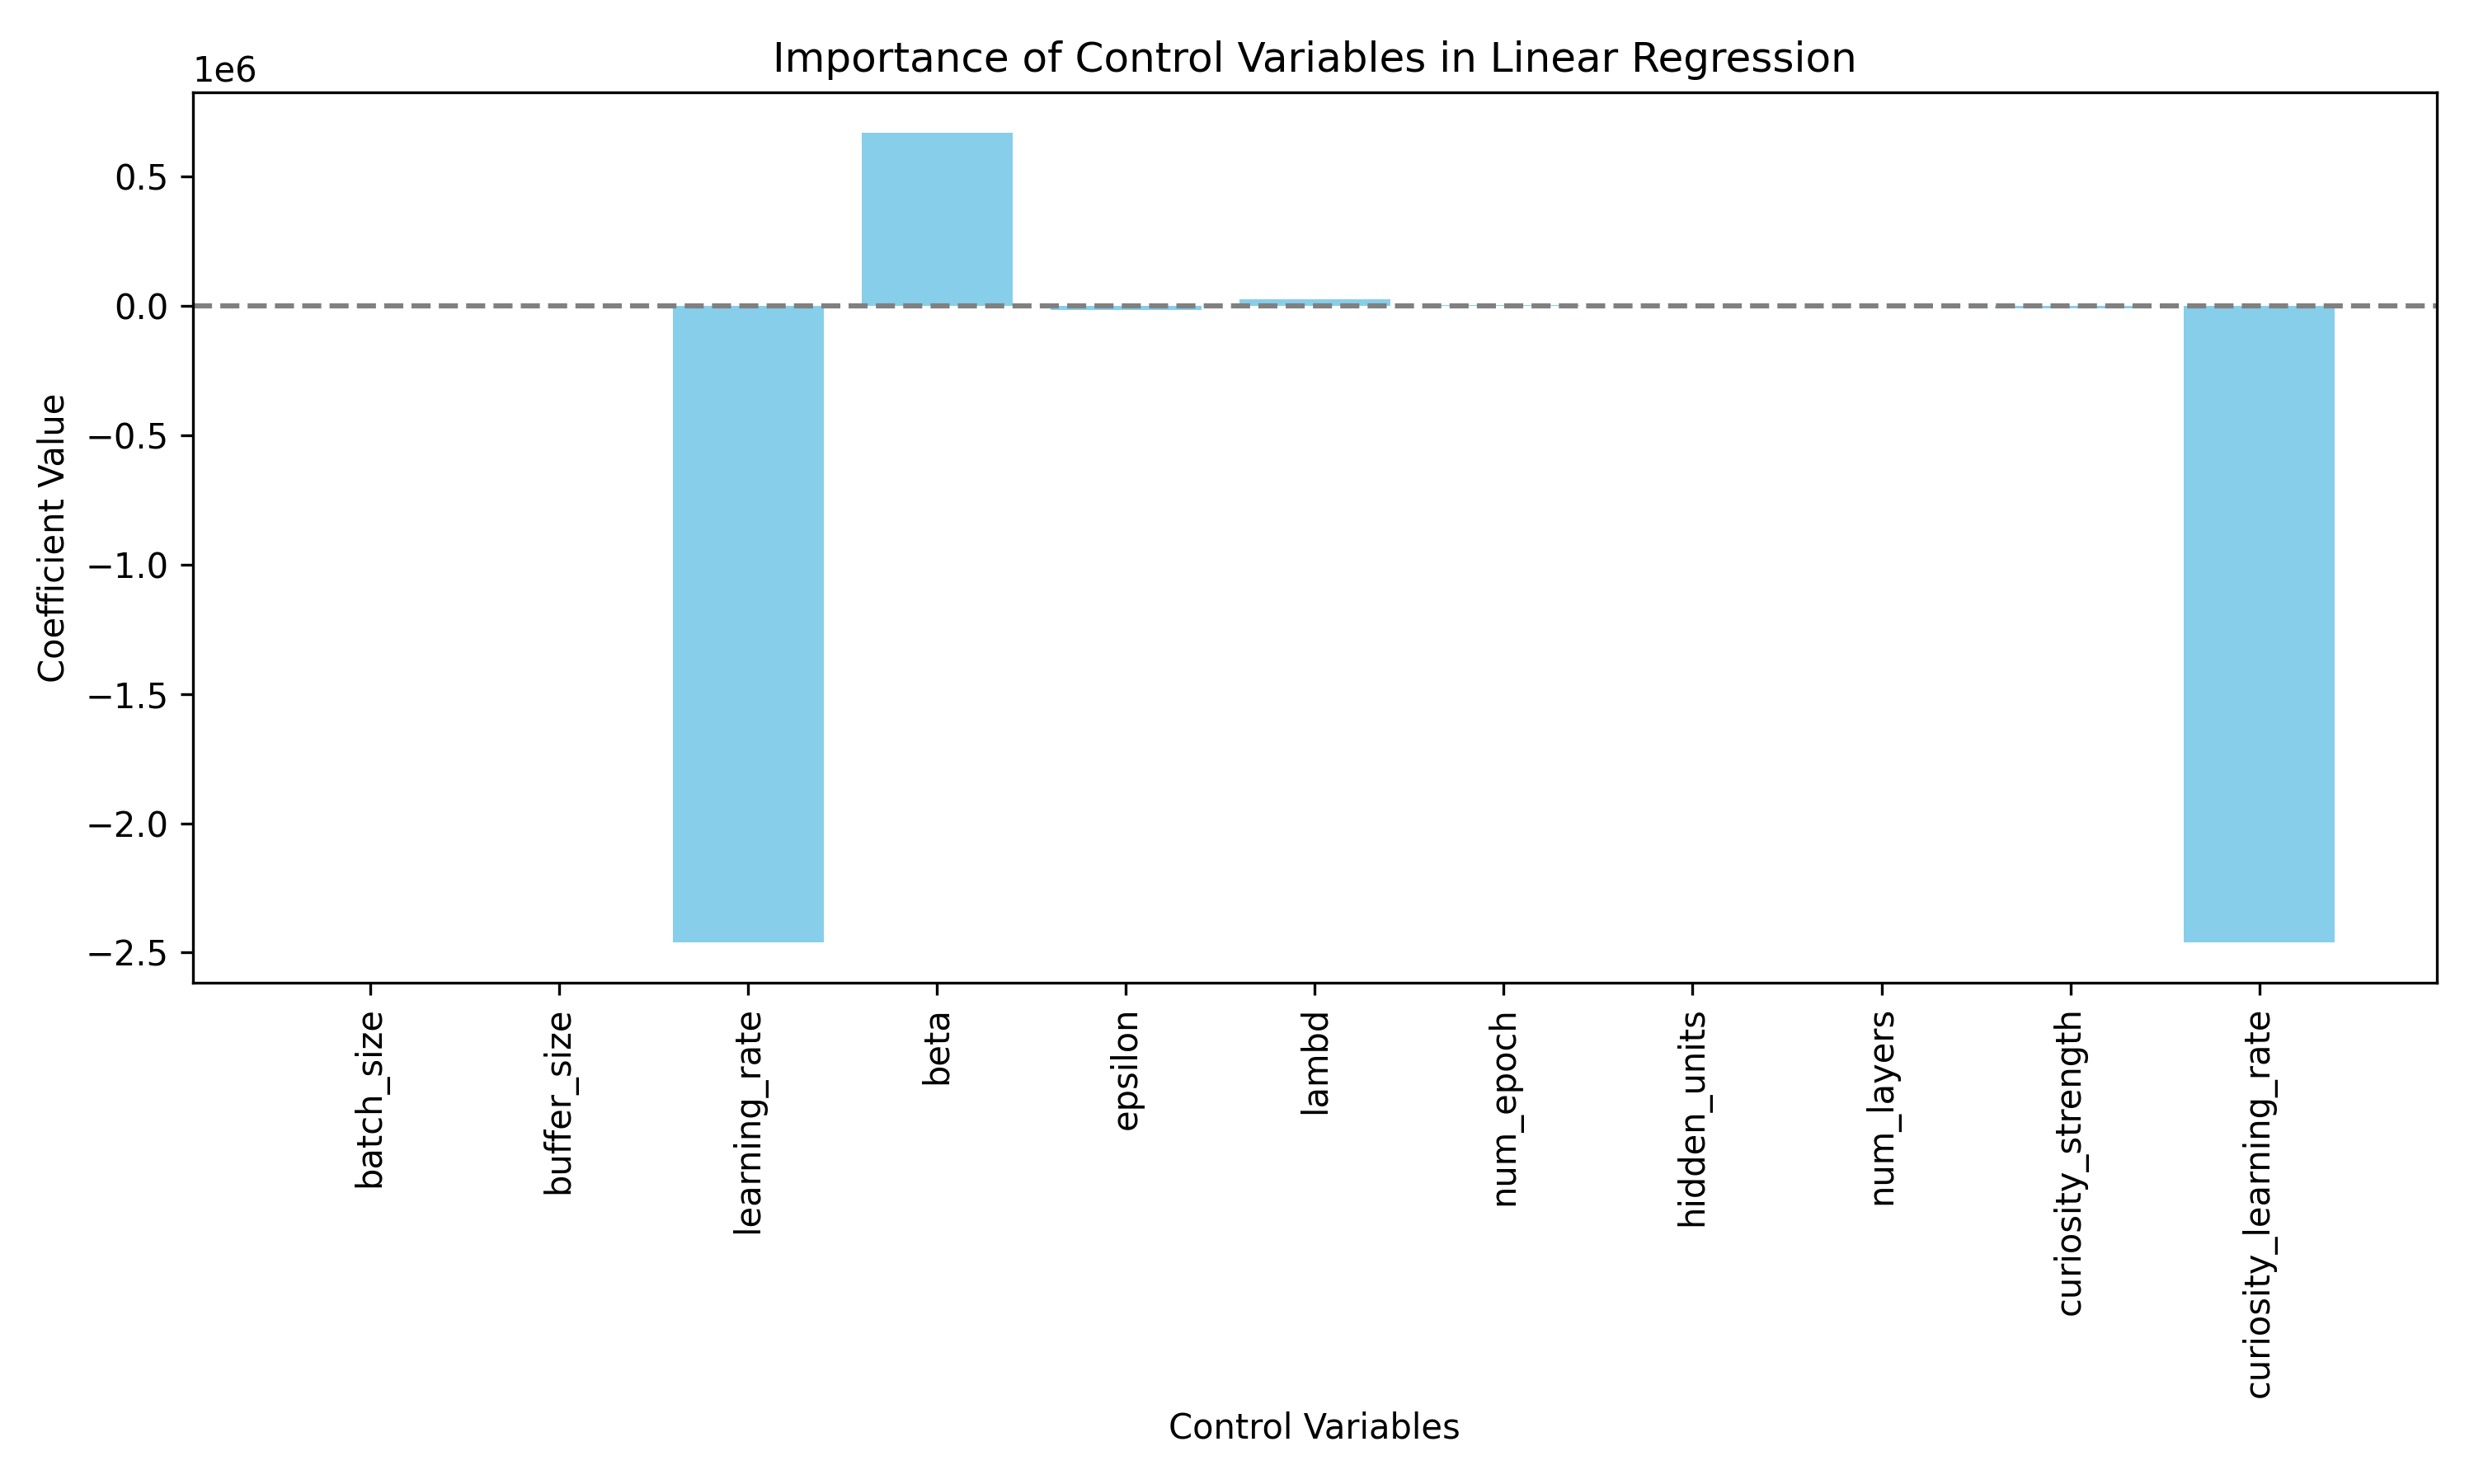
\includegraphics[]{Images/linear_regression_coefficients.png}
%     }
%     \caption{Linear regression model of hyperparameters}\label{regression}
% \end{figure}

\subsection{Final Training}

The final training consisted of 6 different config files, each run for \textit{500,000}, \textit{1,000,000}, \textit{10,000,000} and \textit{30,000,000} steps. Figure$~$\ref{500k_steps} shows the Environment/Cumulative reward for the training runs conducted for 500k steps. It appears the score converges, but on closer inspection it can be seen that all these runs converge on approximately -9.75, which is very far from the theoretical maximum available. This graph suggests these runs were falling into local maxima after learning and didn't have the number of iterations for the curiosity to force the agent to explore beyond this local maxima.
\begin{figure}[!htb]
    \centering
    \resizebox{\textwidth}{!}{%
    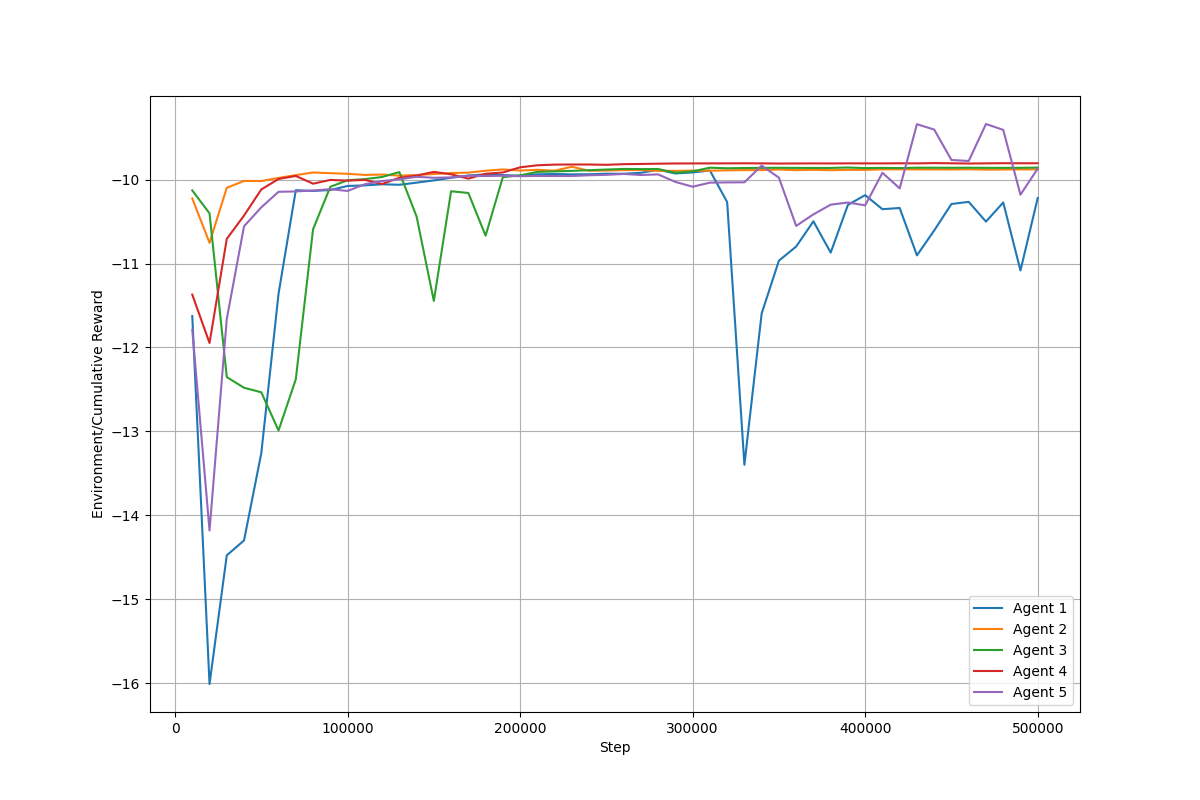
\includegraphics[]{Images/reward_graph_500k.png}
    }
    \caption{Environment/Cumulative reward for 500k steps}\label{500k_steps}
\end{figure}

For the other training runs, it is hard to draw any conclusions about the quality of the training from the model output graphs, shown in section$~$\ref{sec:env_cum_reward} of the appendices, and so all the models were run in heuristic mode in an evaluation scene that logged the performance over time. Several of these models were not even able to control the kiteboat and had completely failed to learn anything. Figure$~$\ref{bad_runs} shows the cumulative reward accumulated over a 90s evaluation run for the 3 models that were unable to control the kiteboat. It can be seen that the cumulative reward never rises as the agents are unable to maintain control of the kiteboat.

\begin{figure}[!htb]
    \centering
    \resizebox{\textwidth}{!}{%
    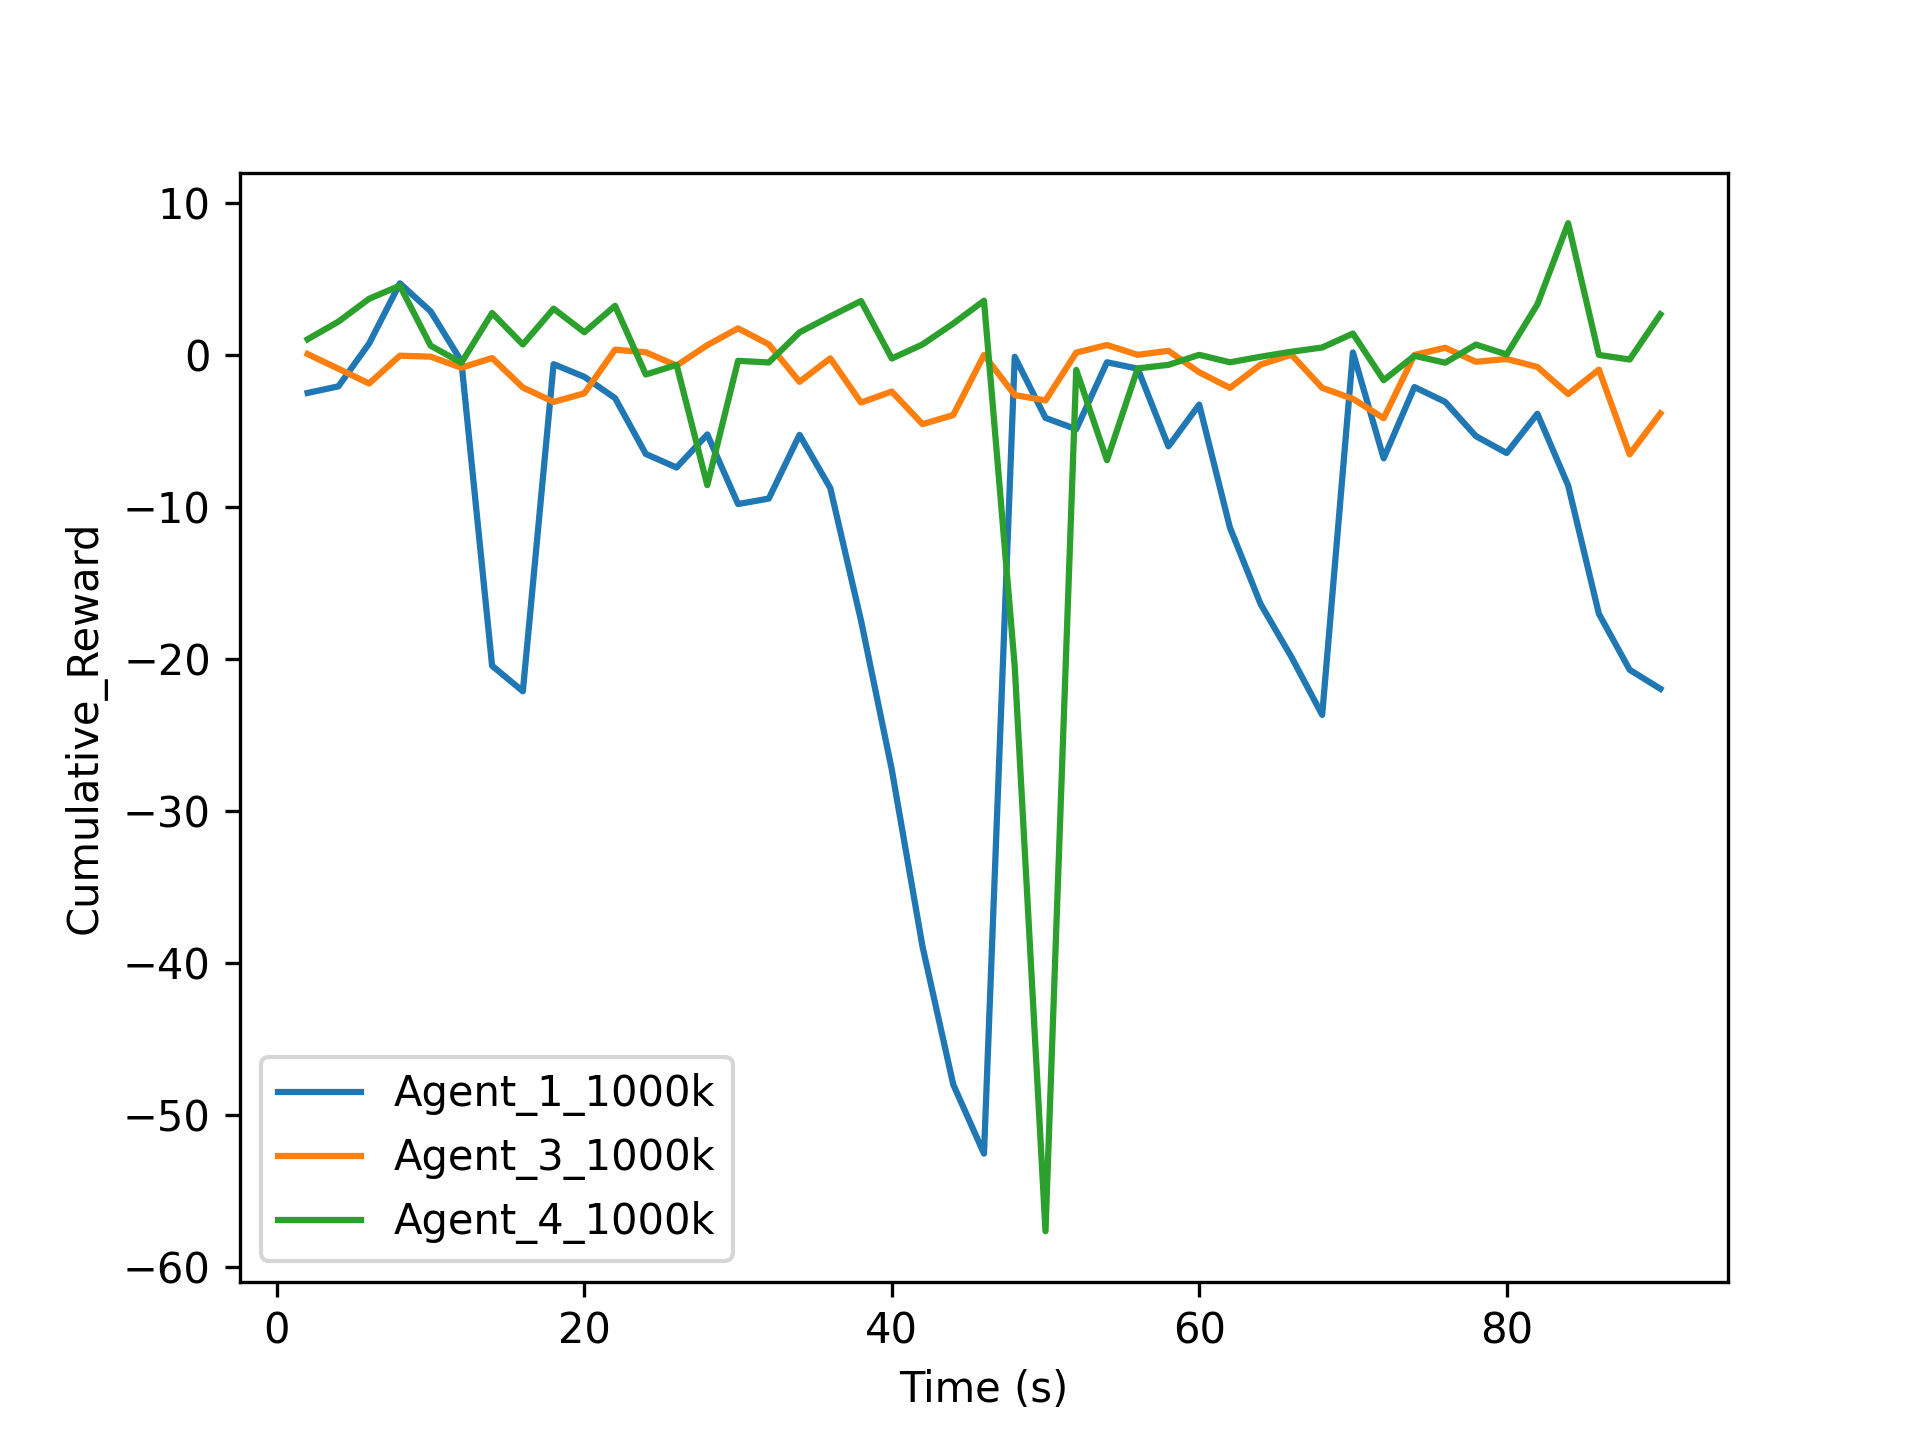
\includegraphics[]{Images/Cumulative_Reward Over Time.png}
    }
    \caption{Cumulative reward of 3 Agents evaluated for 90s}\label{bad_runs}
\end{figure}

The highest performing model was boatAgent\_2 trained for \textit{10,000,000} steps, figure$~$\ref{agent_stats} shows how it performed in the heuristic evaluation given a 300 second time slot. This is the best performing heuristic run of 5 conducted. These figures present the evaluation metrics of \texttt{Cumulative Reward}, \texttt{Completed Waypoints}, \texttt{Distance Covered}, \texttt{Boat Speed}, \texttt{Rudder Angle} and \texttt{Kite Height}. After some initial inconsistency the agent navigated through 3 waypoints, with an average boat speed of 5.05 m/s. Over the course of the evaluation it crashed the kite into the water 6 times. These results show the best performing model was able to sail the kiteboat across a number of waypoints, gaining a large reward and maintaining a good speed, however it was still inconsistent unable to fly the kite reliably for the total duration of the evaluation scene. 
\begin{figure}
    \centering
    \resizebox{\textwidth}{!}{%
    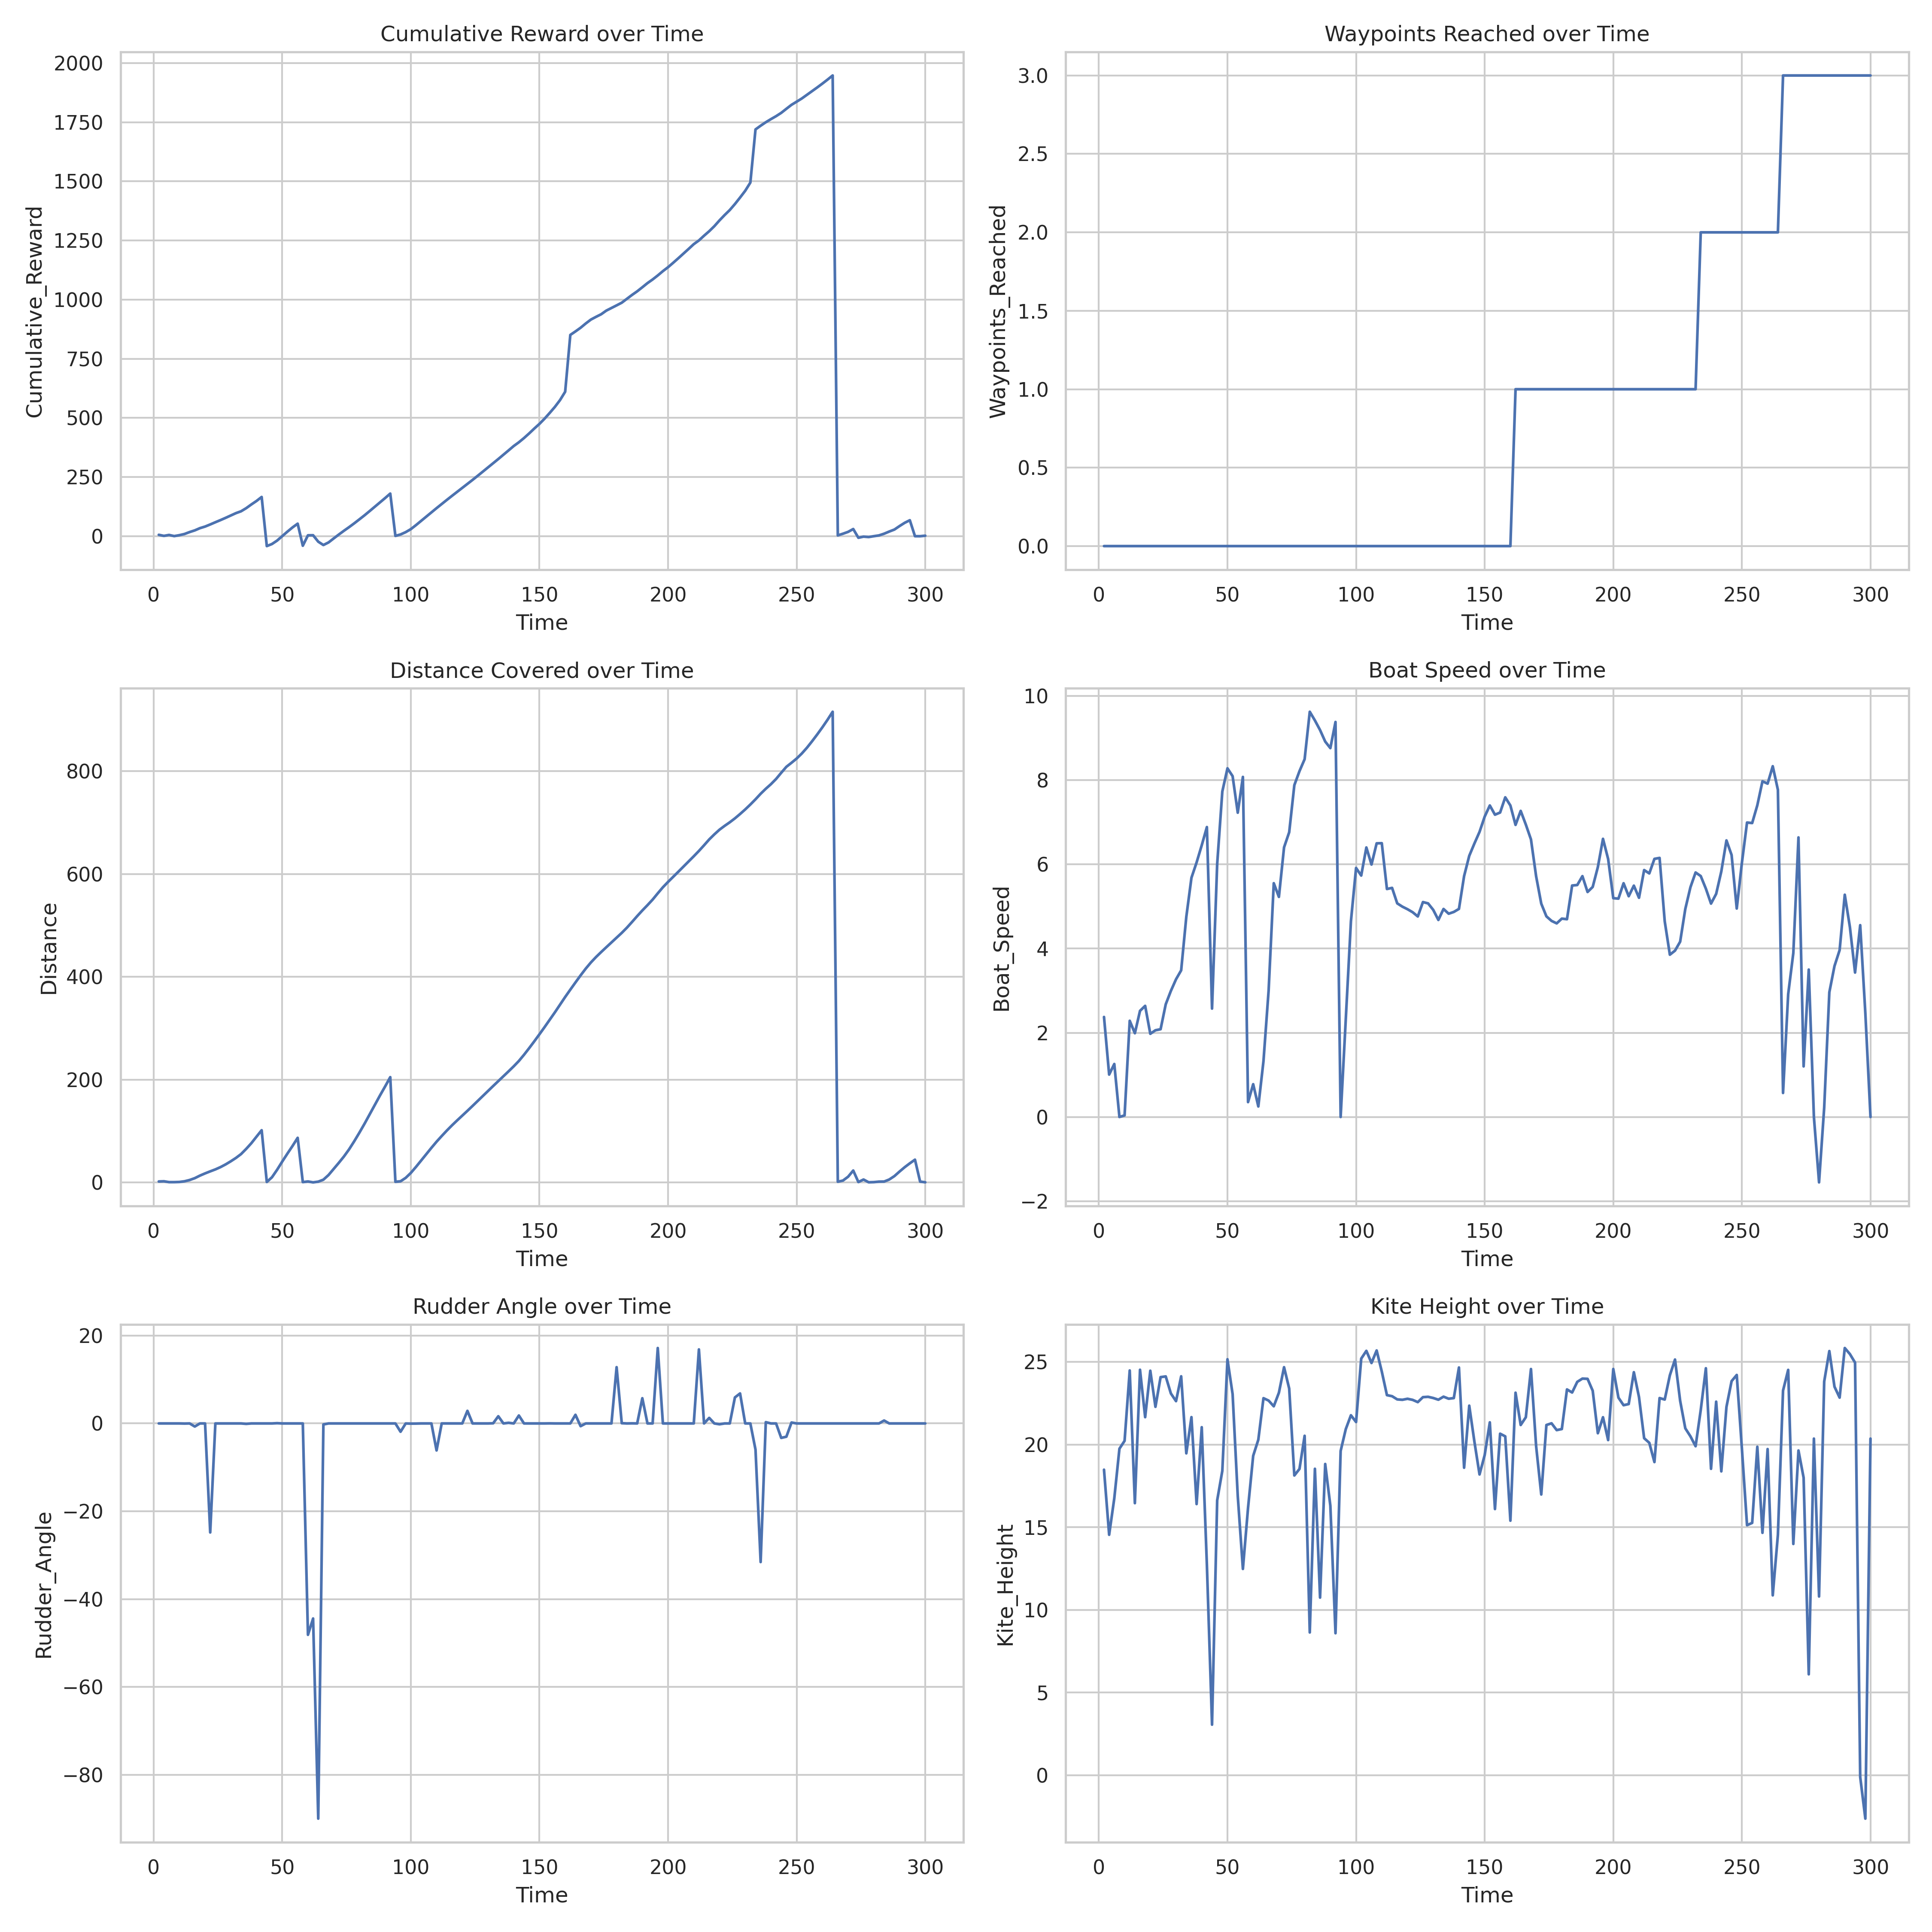
\includegraphics[]{Images/agent_stats.png}
    }
    \caption{Agent stats for 10,000,000 steps model}\label{agent_stats}
\end{figure}

\subsection*{Human Comparison}\label{hcomp}
Earlier it was mentioned that a heuristic playable game was created to make sure the model felt sensible and could be played by a human player. To create a baseline for the agent's performance a human player played the game for 5 minutes in heuristic mode and the results were logged. The top performing agent was then compared against this baseline to see how it performed. The results can be seen in figure$~$\ref{human_comparison}. This figure shows the average \texttt{Cumulative Reward}, \texttt{Distance Traveled}, \texttt{Boat Speed} and {Waypoints Reached} per episode, from the 300s evaluation period. It can be seen that the human outperformed the agent in all catagories

\begin{figure}
    \centering
    \resizebox{\textwidth}{!}{%
    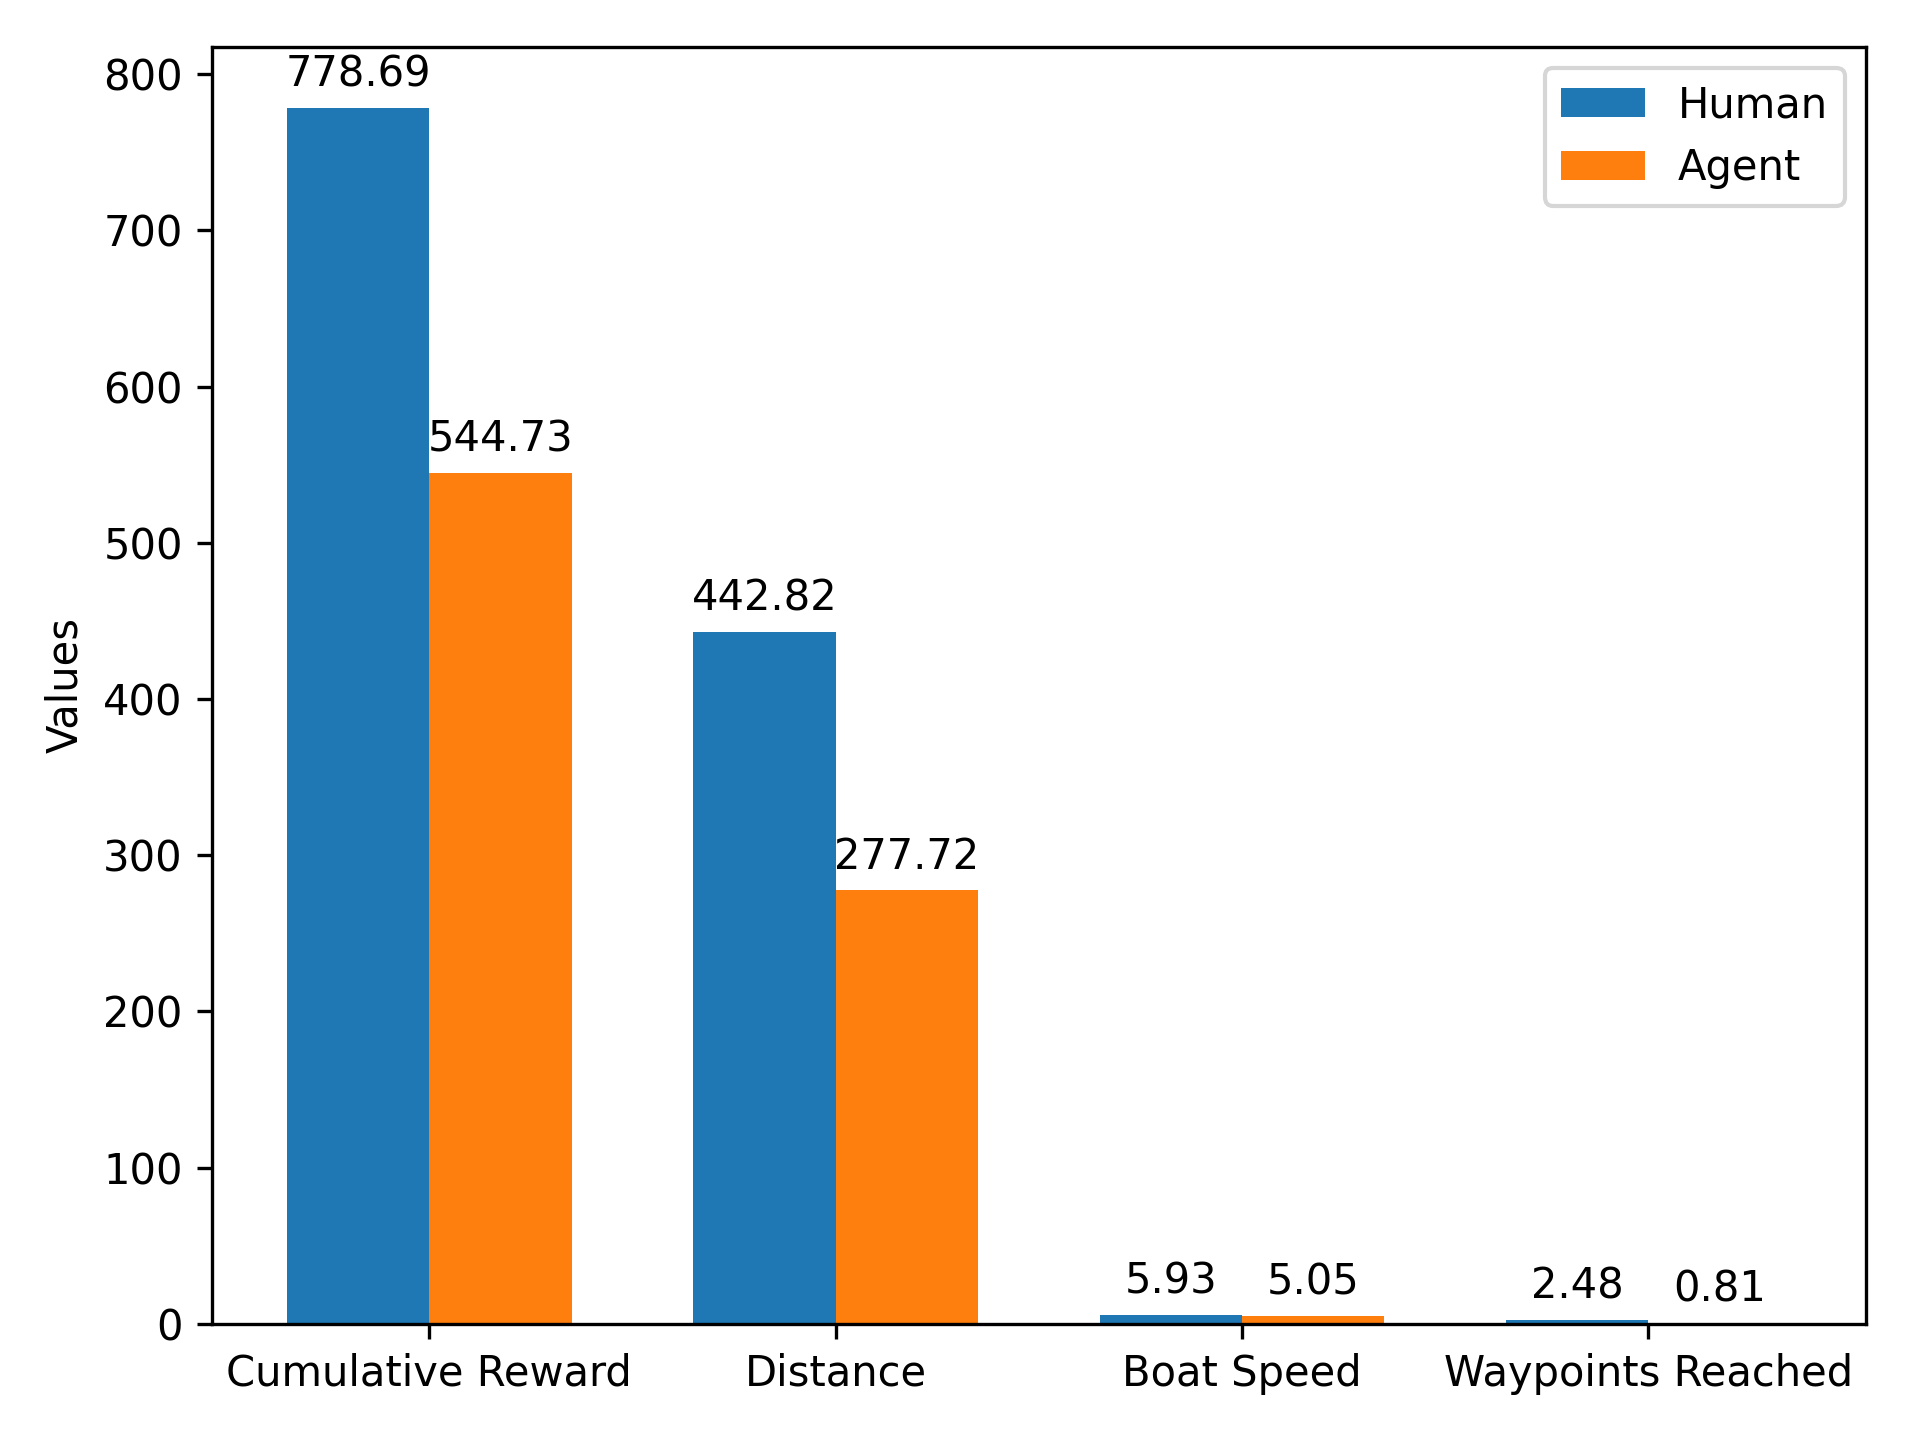
\includegraphics[]{Images/performance_comparison.png}
    }
    \caption{Human comparison vs Model Evaluation}\label{human_comparison}
\end{figure}

\subsection{Hardware}\label{sec:hardware_evaluation}
There were several limitations that affected the quality of the training and thus the trained model. First and foremost was compute, as expected when conducting any machine learning training, the more compute available the better. The local machine used for training was a 16-core i9 with 32GB of RAM and a T2000 nvidia graphics, and took approximately 2 hours per million steps completed. This was not a viable option for training multiple agents to a high level of performance, and so the training was attempted to the university HPC. The HPC has 525 Lenovo nx360 m5 nodes each with two 14 core 2.4 GHz CPUs, and 32 GPU nodes with two cards each. Initially it was anticipated the training should be without issue, this was not quite the case. Unity does not support native multi threading, due to the complex nature of its physics engine, so it runs on a single CPU unless manually specified. Manual threading was possible but only for separate tasks that could be called independently of the model, such as the collision detection algorithm. As expected this severely limits the speed of training, and using the hpc did not radically increase these run times.
However, the HPC was not without its advantages, the main being that it was possible to run multiple training runs in parallel, and so the hyperparameter tuning was conducted on the HPC. This would not have been possible on the local machine as it would have taken far too long to test all the combinations. The ability to submit a large batch of jobs to be run in parallel and then the results collection automated was a huge time saver. The HPC also had the advantage of being able to run the training for longer periods of time without causing inconvenience, so even though the training speed was limited it was not a problem to let them run for many days. 

% The wait time for resources to be allocated increased the longer the job was scheduled to take 


% Thus this project wouldn't have been possible without the HPC.

% The second more major problem was the wait time of the HPC, the longer a job was scheduled the longer it took for the resources to be allocated, for a job that was scheduled for 48 hours on a single node it could take up to 5 days for the job to begin. This was a major problem as it meant that the training could not be conducted in a timely manner, and iteration was very slow. The limited GPU's had the same problem, with only 32 available, and the fact that the HPC was shared with the entire university, it was very difficult to get access to the resources. For this reason the vast majority of training was conducted on the local machine, which had the advantage of also being able to see the training in real time, albeit slowly.   


\section{Agent Performance}

\subsubsection*{Difficulties Encountered}
There were several difficulties encountered when trying to get the agent to learn anything let alone the combination of directionally sailing a kiteboat. One of the most common local maxima that the agent fell into was to steer on `hard lock' with the rudder at \textit{$\tilde{} ~70-90^{\circ}$}, shown in figure$~$\ref{hard_lock} where the target can be seen as the green area in the distance. This behaviour allowed it to learn to fly the kite very reliably with the boat in a more consistent and stable position. These episodes provided false positives in the training data because as soon as the agent started to explore the rudder space more it was not able to fly the kite. To try and combat this behaviour a large negative reward was added for aggressive steering as shown in table$~$\ref{rewards}. This went some way to discouraging this behaviour but it was still observed in some of the later training runs. After this rudder reward was added it was observed that the agent took almost 5 times as long to learn to fly the kite with some reliability. 
\begin{figure}[!htb]
    \centering
    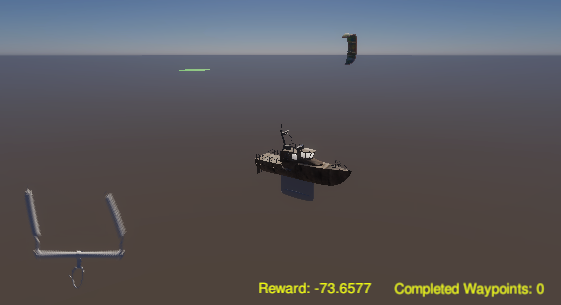
\includegraphics[width=0.8\textwidth]{Images/hard_lock.png}
    \caption{The agent steering on hard lock}\label{hard_lock}
\end{figure}

\subsection*{Performance in Curriculum}
While the agent showed promise in its basic understanding and control, it was unable to progress sufficiently through the training curriculum. The curriculum, which was designed to gradually increase in complexity, required the agent to reliably control of the kiteboat if it wanted to progress to the next stages, including sailing upwind. The agent's overall inconsistent performance in kite control hindered its progression, preventing it from reaching these more advanced stages.


\section{Practical Deployment}\label{sec:practical_deployment}
The results of the model demonstrate unreliability in the agents performance and so it would not be recommended to deploy this particular model into the real world. However, the results do show promise and it is likely possible to create a model that performs reliably enough to warrant building a physical prototype. Integration into a physical system would first require a boat and kite. The boat would need to be large enough to safely contain all the components (including electrics) so a vessel of appropriately 18 - 30ft would be advised. For the kite a standard off the shelf LEI kite would perform fine, the size of the kite could be changed depending on the wind conditions it would be tested in as it wouldn't noticeably affect the handling. The remainder of the system would involve addressing the following design and manufacture points:  

\begin{itemize}
    \item Kite Control System:
    \begin{itemize}
        \item Custom reinforced attachment point to the boat. Similar to a mast base attachment point.
        \item Electronic winches for kite line management.
        \item Load cells for tension measurement in kite lines.
        \item Gyroscopic sensors to measure kite orientation.
        \item Anemometer for wind speed and direction data.
        \item Manual override for emergency control.
    \end{itemize}
    \item Rudder Control System:
    \begin{itemize}
        \item Electric linear actuators
        \item Rudder position sensor
        \item Manual steering mechanism
    \end{itemize}
    \item Central Processing Unit
    \begin{itemize}
        \item Microcontroller to run the control system.
        \item Data acquisition system (DAQ) to interface with sensors and actuators.
        \item GPS module for positioning.
        \item Compass module for heading data.
    \end{itemize}
    \item Power Supply
    \begin{itemize}
        \item Battery bank with charge controller.
        \item Solar panels for charging.
    \end{itemize}
\end{itemize}

A visual breakdown of how this system would come together is shown in figure$~$\ref{physical_kiteboat}. Addressing these points would lead to an mvp capable of testing. It is important to note that all the observations provided to the agent in the simulation must still be provided to the trained model, so the same observations would have to be collected.

\begin{figure}
    \centering
    \resizebox{\textwidth}{!}{%
    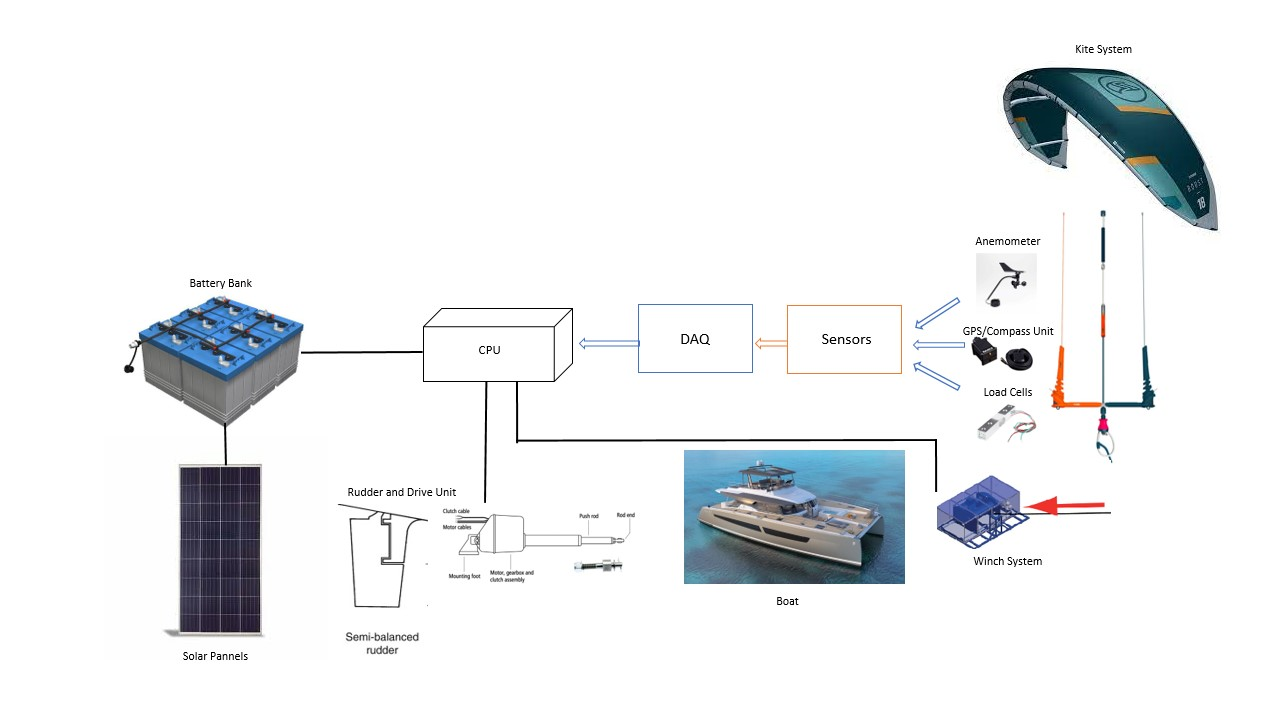
\includegraphics[width=0.8\textwidth]{Images/Slide1.jpg}
    }
    \caption{Physical kiteboat system}\label{physical_kiteboat}
\end{figure}

\section{Critical Evaluation}
The overarching aim of this research paper was to develope a system for autonomously controlling a kite-powered vessel using reinforcement learning. Tables$~$\ref{obj1} - explores the extent to which this aim was achieved by investigating the success of each objective and its outcome goal. To evaluate each objective in detail a score was assigned from 0 to 10, with the range shown in figure$~$\ref{score_range}. A total score was calculated for each objective and its value discussed.
\newline
\begin{chronology}[5]{0}{9}{\textwidth}
    \event{0}{Failed}
    \event{5}{Satisfactory}
    \event{10}{Best Result}
\end{chronology}\label{score_range}

\begin{table}[!htb]
    \centering
    \resizebox{\textwidth}{!}{%
    \begin{tabular}{p{0.8\textwidth}|c}
        \textbf{Objective 1: Simulation Environment Development} & \textbf{Score} \\
        \hline
         To design and implement a virtual marine environment that accurately emulates real-world maritime conditions. & 9 \\
        \midrule
        To construct a realistic model of a boat that exhibits appropriate physical movements in response to environmental forces such as wind and water currents. & 7 \\
        \hline
        \textbf{Outcome Goal(s)} &  \\
        \midrule
        To have a physics-based boat able to be controlled and driven around a scene by a human player. & 10 \\
        \midrule
        \textbf{Total} & \textbf{$\frac{26}{30}$} \\
        \bottomrule
    \end{tabular}
    }
    \caption{Objective 1 Evaluation}\label{obj1}
\end{table}

Objective 1 scored a total of $\frac{27}{30}$, the Unity environment implemented was capable of delivering real world conditions with a variety of wind and waves. The boat model was able to be accurately controlled by a human player and experienced buoyant and drag forces. There was room for improvement within the boat model by implementing a custom particle simulation instead of the Unity water system, which would have provided complete control over the interaction between the water and the boat. 

\begin{table}[!htb]
    \centering
    \resizebox{\textwidth}{!}{%
    \begin{tabular}{p{0.8\textwidth}|c}
        \textbf{Objective 2: Kite Propulsion Modeling} & \textbf{Score} \\
        \hline
        To create a physics-based model of a kite within the simulation that reflects authentic aerodynamic behaviours and integrate it onto the boat model. & 5 \\
        \midrule
        To integrate kite control mechanics into an agent’s available action space. & 9 \\
        \hline
        \textbf{Outcome Goal(s)} &  \\
        \midrule
        To have a physics-based kiteboat able to be controlled and driven around a scene by a human player, using an agent's heuristic controls. & 10 \\
        \midrule
        \textbf{Total} & \textbf{$\frac{25}{30}$} \\
        \bottomrule
    \end{tabular}
    }
    \caption{Objective 2 Evaluation}\label{obj2}
\end{table}

Objective 2 scored a total of $\frac{24}{30}$, shown in table$~$\ref{obj2}, the physics of the kite model were satisfactory. The kite generated a resultant force that was capable of pulling the boat and the outcome goal was fully achieved. However there was definitely room for improvement in the kite model, specifically in how the kite rotated. To keep the model simple a torque was applied to the kite about the centre of mass, this was not a realistic representation of how a kite would rotate. A more realistic approach would have been to apply a torque about the point on the wingtip of the kite, switching left/right depending on the direction of turn. Even better than this would be to create a kite model that didn't rely on the assumption that wind was laminar over the entire kite. This would have allowed for non uniform lift over the kite giving it a realistic rotation behaviour. That being said that model employed in this project was sufficient. The kite controls were successfully placed into discrete actions that the agent could control, it would have been interesting to experiment further with continuous actions, but this would have also increased the complexity of the already difficult learning task.

\begin{table}[!htb]
    \centering
    \resizebox{\textwidth}{!}{%
    \begin{tabular}{p{0.8\textwidth}|c}
        \textbf{Objective 3: Reinforcement Learning Framework Establishment} & \textbf{Score} \\
        \hline
        To formulate a set of observations, actions, and rewards that encapsulate the dynamics of autonomous kite-boat control and navigation. & 9 \\
        \midrule
        To deploy the Proximal Policy Optimisation algorithm, leveraging its actor-critic method for effective policy learning. & 8 \\
        \hline
        \textbf{Outcome Goal(s)} &  \\
        \midrule
        To have an agent begin training using PPO to learn to control the kiteboat. & 10 \\
        \midrule
        \textbf{Total} & \textbf{$\frac{27}{30}$} \\
        \bottomrule
    \end{tabular}
    }
    \caption{Objective 3 Evaluation}\label{obj3}
\end{table}

Objective 3 scored a total of $\frac{27}{30}$, shown in table$~$\ref{obj3}, the observations, actions, and rewards were all successfully formulated and the agent was able to begin training. The observations and rewards were tuned through lots of trial and error in an attempt to create a stable system for the agent to learn. The PPO algorithm was successfully implemented and the agent was able to train.

\begin{table}[!htb]
    \centering
    \resizebox{\textwidth}{!}{%
    \begin{tabular}{p{0.8\textwidth}|c}
        \textbf{Objective 4: Autonomous Agent Development} & \textbf{Score} \\
        \hline
        To develop an RL agent capable of learning basic control and maneuvers, starting with simple navigating towards a target and maintaining a constant course. & 8 \\
        \midrule
        To refine the agent's capability to adaptively control the kite's position and angle to optimise propulsion for speed while navigating towards a target. & 5 \\
        \hline
        \textbf{Outcome Goal(s)} &  \\
        \midrule
        To have an agent that can navigate towards a target in a straight line. & 8 \\
        \midrule
        To have an agent that can navigate towards a target in any direction, including using maneuvers to take the optimal path. & 0 \\
        \midrule
        \textbf{Total} & \textbf{$\frac{21}{40}$} \\
        \bottomrule
    \end{tabular}
    }
    \caption{Objective 4 Evaluation}\label{obj4}
\end{table}
Objective 4 scored a total of $\frac{21}{40}$, shown in table$~$\ref{obj4}, the agent was capable of learning the controls of the kiteboat, and able to reliably fly the kite and steer. It was at this point where the complexity of the task started to limit the agents progression through the curriculum. Reliability was a problem when attempting to optimise for speed, the agents performance was inconsistent meaning that on occasion it was able to maintain control and attempt to navigate towards several waypoints as discussed in section$~$\ref{hcomp}, but this was not consistent enough to progress through the curriculum and learn to sail upwind. As a result the model was not able to navigate in any direction. It is likely that this control problem is well within the capabilities of RL and the PPO algorithm, but the complexity of the task necessitated a more realistic model, more complex reward function and better hyperparameter tuning. Objective 4 was not fully achieved, but the agent was able to learn the controls of the kiteboat and navigate towards a target in a straight line.  

\begin{table}[!htb]
    \centering
    \resizebox{\textwidth}{!}{%
    \begin{tabular}{p{0.8\textwidth}|c}
        \textbf{Objective 5: Efficacy and optimisation Testing} & \textbf{Score} \\
        \hline
        To utilise High-Performance Computing (HPC) resources for scaling up simulations and optimising the training process. & 8 \\
        \midrule
        To rigorously evaluate the trained agent’s performance in simulating autonomous navigation in various environmental scenarios. & 8 \\
        \hline
        \textbf{Outcome Goal(s)} &  \\
        \midrule
        To train an agent using the HPC resources. & 8 \\
        \midrule
        To have an agent that can navigate towards a target in a straight line under various environmental conditions, including wind and waves. & 2 \\
        \midrule
        \textbf{Total} & \textbf{$\frac{26}{40}$} \\
        \bottomrule
    \end{tabular}
    }
    \caption{Objective 5 Evaluation}\label{obj5}
\end{table}

Objective 5 scored a total of $\frac{26}{40}$, shown in table$~$\ref{obj5}. The HPC was used extensively for training a large number of models, but it does not warrant a full score as it was not used with any in depth parallelisation strategies, merely single runs on single nodes. The trained agents were run in the evaluation scene and compared against human baselines, testing all the learnt behaviours and scoring them appropriately. It would have been exciting to pit multiple agents against one another during the evaluation for a direct comparison, but this remains future work. The agent was able to navigate towards a target in a straight line, and was still able to do so under changing sea states. The wind was not changed during the evaluation as the agent was only trained on laminar wind and never progressed to the stages of changing weather conditions.

\begin{table}[!htb]
    \centering
    \resizebox{\textwidth}{!}{%
    \begin{tabular}{p{0.8\textwidth}|c}
        \textbf{Objective 6: Real-World Applicability Assessment} & \textbf{Score} \\
        \hline
        To extrapolate simulation findings to assess real-world applicability and propose a  practical deployment of RL in kite-powered vessels. & 8 \\
        \midrule
        To provide recommendations for further research and development based on empirical results obtained from the simulation studies. & 8 \\
        \midrule
        \textbf{Total} & \textbf{$\frac{16}{20}$} \\
        \bottomrule
    \end{tabular}
    }
    \caption{Objective 6 Evaluation}\label{obj6}
\end{table}

Objective 6 scored a total of $\frac{16}{20}$, shown in table$~$\ref{obj6}. A practical deployment of the kiteboat was considered in section$~$\ref{sec:practical_deployment}, although there is likely to be a significant amount of work to build a physical prototype. Other considerations such as where to test the mvp, and how to ensure safety would need to be addressed. The recommendations for further research and development are discussed in Chapter$~$\ref{chap:future_work}. 


After the evaluation of the objectives and their outcome goals a final score of $\frac{141}{180}$ was achieved, which equates to 78.3\%. This score is an individual evaluation of the performance of the system against the specified objectives and so is not a direct score of how well the system performs as a whole, merely how close it came to meeting the goals set out at the start of the project. 
